\documentclass{article}
\usepackage[english]{babel}
\usepackage[letterpaper,top=2cm,bottom=2cm,left=2.5cm,right=2.5cm,marginparwidth=1.25cm]{geometry}

\usepackage{hyperref, booktabs, float}
\usepackage[leqno]{amsmath}
\usepackage{enumitem, nccmath,lipsum,amssymb,xcolor,xparse,listings, blindtext,verbatim}
\usepackage[most]{tcolorbox}

\usepackage{graphicx}
\graphicspath{ {./attachments/} }

\NewDocumentCommand{\codeword}{v}{\texttt{\textcolor{blue}{#1}}}

\definecolor{light-gray}{gray}{0.95}
\newcommand{\code}[1]{\colorbox{light-gray}{\texttt{#1}}}


\lstset{language=C, keywordstyle={\bfseries \color{blue}}}

\NewDocumentCommand{\mynote}{+O{}+m}{%
  \begingroup
  \tcbset{%
    noteshift/.store in=\mynote@shift,
    noteshift=1.5cm
  }
  \begin{tcolorbox}[nobeforeafter,
    enhanced,
    sharp corners,
    toprule=0.5pt,
    bottomrule=0.5pt,
    leftrule=0pt,
    rightrule=0pt,
    colback=green!10,
    #1,
    left skip=\mynote@shift,
    right skip=\mynote@shift,
    overlay={\node[right] (mynotenode) at ([xshift=-\mynote@shift]frame.west) {\textbf{Note:}} ;},
    ]
    #2
  \end{tcolorbox}
  \endgroup
  }
\makeatother

\newcommand{\mytext}[1]% #1 = same as intertext
{&\parbox{0.9\textwidth}{\rule{0pt}{.5\baselineskip}\\
\textrm{#1}\\
\rule{0pt}{.5\baselineskip}}&\\}

\newcounter{exercise}
\newcounter{problem}[exercise]
\newcommand{\myitem}{\stepcounter{problem}\tag*{\alph{problem})}}

\title{Lab 5: Processes and signals}
\author{Mashenkov Timofei B23-CBS-02 \\ \href{mailto:t.mashenkov@innopolis.university}{t.mashenkov@innopolis.university}}
\begin{document}
\maketitle{}

\section{What are zombie processes? How can you find and kill them?}
\noindent

\begin{itemize}
	\item Zombie processes are terminated processes that remain in the process table because their parent has not done cleanup (reaped them). They consume no resources but may exhaust available process IDs if left unchecked.
	\item \textbf{How to find them?} \code{ps -aux | grep Z} or \code{ps wauxf | less} \\ 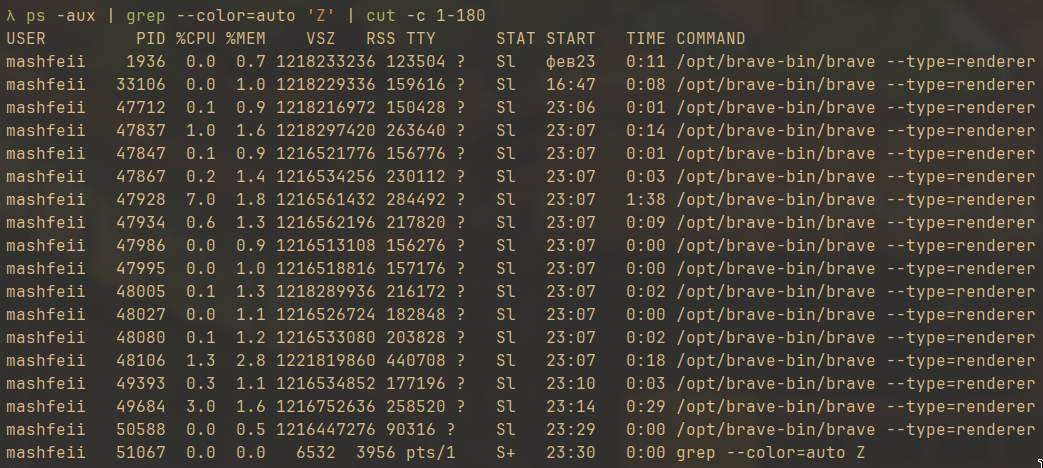
\includegraphics[width=460pt]{5_1.jpg}
	\item \textbf{How to kill them?}
	      \begin{itemize}
		      \item \code{kill -s SIGCHLD <PARENT\_PID>} - tell parent to perform cleanup
		      \item \code{kill -9 <PARENT\_PID>} - kill parent if it doesn't respond
		      \item reboot the system
	      \end{itemize}
\end{itemize}

\section{Differences between \code{kill}, \code{killall}, and \code{pkill}}
\noindent

\begin{itemize}
	\item \code{kill}: Terminates processes by PID. Requires specifying the signal (e.g., \code{kill -9 228}).
	\item \code{killall}: Terminates processes by name (e.g., \code{killall -SIGTERM brave}).
	\item \code{pkill}: Uses patterns to match process names or attributes (e.g., \code{pkill -f "sleep"}).
\end{itemize}

\section{\code{top}'s \code{Tasks} and \code{\%Cpu(s)} lines}
\noindent

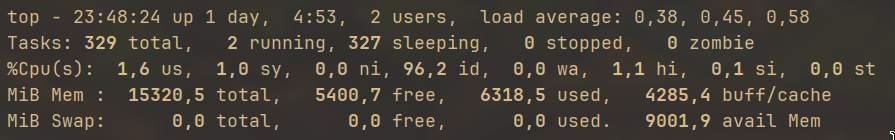
\includegraphics[width=460pt]{5_2.jpg}

\begin{itemize}
	\item \code{Tasks}:
	      \begin{itemize}
		      \item \code{329 total}: Total processes
		      \item \code{2 running}: Processes actively using CPU
		      \item \code{327 sleeping}: Processes waiting for resources
		      \item \code{0 stopped}: Processes paused (e.g., via SIGSTOP)
		      \item \code{0 zombie}: Terminated but un-reaped processes
	      \end{itemize}
	\item \code{\%Cpu(s)}:
	      \begin{itemize}
		      \item \code{us}: User-space CPU usage
		      \item \code{sy}: Kernel-space CPU usage
		      \item \code{id}: Idle CPU percentage
		      \item \code{wa}: CPU waiting for I/O operations
		      \item \code{hi/si}: Hardware/software interrupt overhead
		      \item \code{st}: Virtual CPU time lost due to hypervisor
	      \end{itemize}
\end{itemize}

\section{Bash script to kill "random" processes}
\noindent

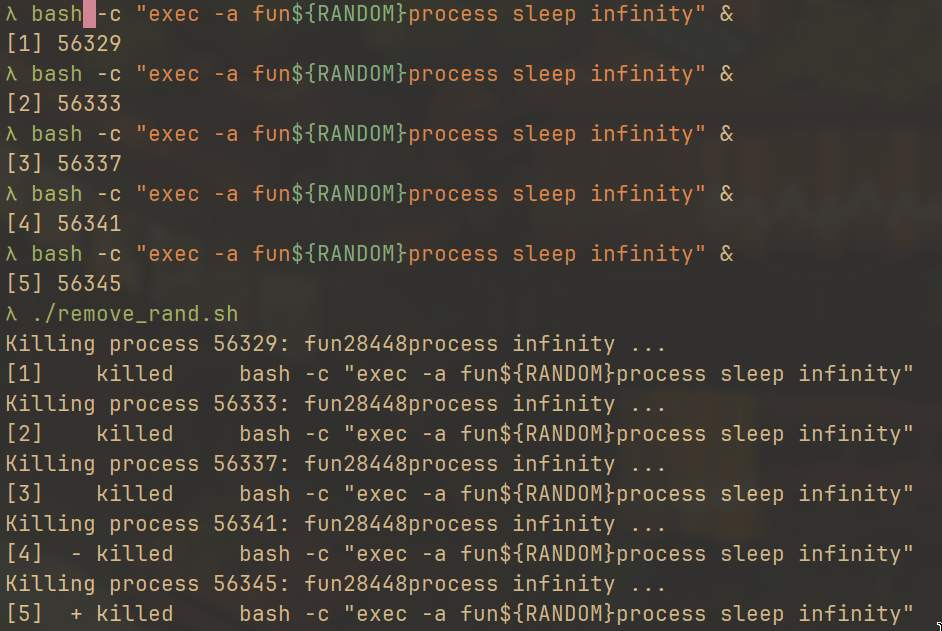
\includegraphics[width=460pt]{5_4.jpg}

\section{Script "Hello, world!"}
\noindent

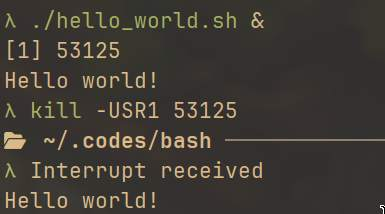
\includegraphics[width=180pt]{5_5.jpg}

\section{Script to system monitor and log into a file}
\noindent

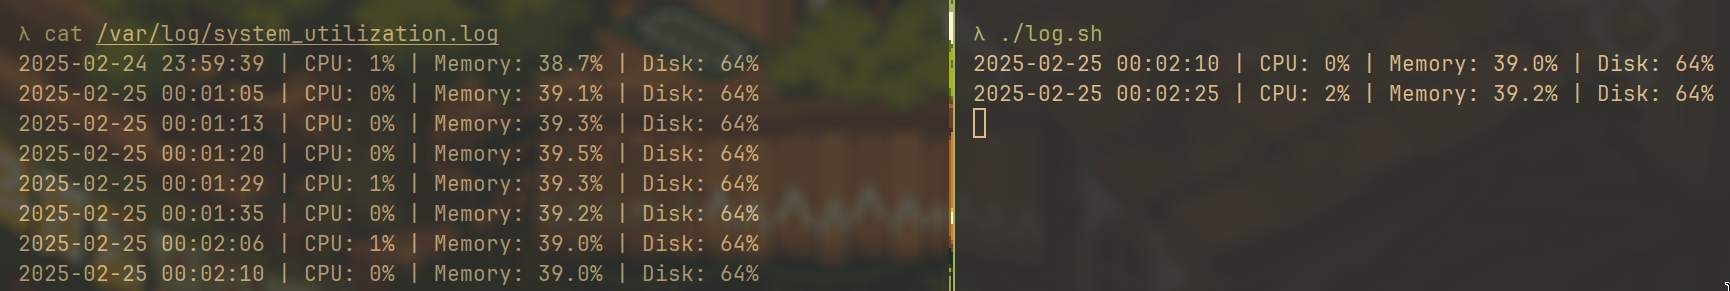
\includegraphics[width=460pt]{5_6.jpg}

\end{document}
